\begin{figure}[htbp]
	\centering
	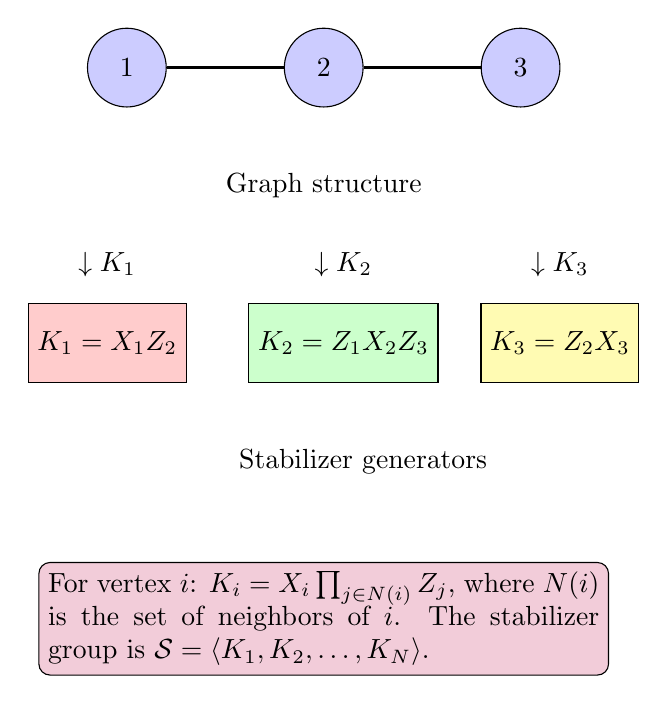
\begin{tikzpicture}
		\node[draw, circle, fill=blue!20, minimum size=1cm] (1) at (-1,0) {1};
		\node[draw, circle, fill=blue!20, minimum size=1cm] (2) at (1.5,0) {2};
		\node[draw, circle, fill=blue!20, minimum size=1cm] (3) at (4,0) {3};

		\draw[thick] (1) -- (2) -- (3);

		\node at (1.5,-1.5) {Graph structure};

		\node at (-1.25,-2.5) {$\downarrow K_1$};
		\node at (1.75,-2.5) {$\downarrow K_2$};
		\node at (4.5,-2.5) {$\downarrow K_3$};

		\node[draw, rectangle, fill=red!20, minimum height=1cm] at (-1.25,-3.5) {$K_1 = X_1 Z_2$};
		\node[draw, rectangle, fill=green!20, minimum height=1cm] at (1.75,-3.5) {$K_2 = Z_1 X_2 Z_3$};
		\node[draw, rectangle, fill=yellow!30, minimum height=1cm] at (4.5,-3.5) {$K_3 = Z_2 X_3$};

		\node at (2.0,-5) {Stabilizer generators};

		\node[draw, rounded corners, fill=purple!20] at (1.5,-7) {
			\begin{minipage}{7cm}
				For vertex $i$: $K_i = X_i \prod_{j \in N(i)} Z_j$, where $N(i)$ is the set of neighbors of $i$. The stabilizer group is $\mathcal{S} = \langle K_1, K_2, \ldots, K_N \rangle$.
			\end{minipage}
		};
	\end{tikzpicture}
	\caption{Reading stabilizer generators from the graph structure. For each vertex $i$, the stabilizer generator $K_i$ is the product of $X$ on vertex $i$ and $Z$ on all its neighbors. These $N$ operators generate the full stabilizer group of $2^N$ elements.}
	\label{fig:stabilizer-generators}
\end{figure}
